\section{Implementation}

%Here you can place more technical details. Are you using Qt, OpenGL, CUDA (which version), shaders, pthreads, etc. What type of graphics hardware were you using? Did you use third party packages? Describe them here. 

%Did you need to take any shortcuts due to time with respect to your design? What are the limitations of your implementation. 

Both Qt and OpenGL were essential to the implementation of this project. QT was used to create 
the GUI and animation, and all programming was completed in C++.

As mentioned in the design secion, two different shaders were needed in the implementation 
of this simulation.
The first shader is used for the particle system and the second shader is used for the cube. 
While the vertex shaders for each are very similar and include simple information about the
position of points and the camera, the fragment shaders implementation are different.  The fragment
shader for the cube is a simple shader that only colors applies color, while the
fragment shader for the particles is more complex and includes ambient, specular, and diffuse
lighting. Two different paint functions were also implemented: one to deal with the static
scene and one to deal with the particles.

Writing information to the VBO was another key element of our implementation that we were
previously inexperienced with. Specifically, we had to store the position information for 
all the particles for a given time step to a temporary array and then write this informaiton
to the VBO at once. Each time the positions were updated, the information sent to the VBO
had to be overwritten. The shaders were then responsible for interpretting this information
and drawing the scene.

The octree was a key element of our implementation because it greatly improved the runtime 
and performance. Octrees work by recursively subdividing the space into eight regions untill
a specified depth isreached. We use a depth of five because we experimentally found this
worked well with the number of particles we use. Octrees can be used in various graphics
applications for spatial 
representaiton. Our application, and a common one for octrees, is collision detection.
When we want to detect if a particle is in collision with any other particle, we check 
the boundaries of that particle with all other particles that exist within the same
octree node because particles that exist within an octree node are close together.
This allows us to dramatically reduce the amount of particles that 
are in possible collision with our current particle.

To find out if two particles within the same octree node are in collision, the following check is run:
\begin{align*}
  & if \: (P_1 - P_2)^2 < (4*radius*radius) \\
  & and \: \Delta V \cdot \Delta R < 0 \: then \: collision
\end{align*}

If indeed two particles are in collision then the updated velocities are as follow:
\begin{align*}
  &  V_1 = \mu [V_1 - 2*\Delta R*(V_1\cdot \Delta R)] \\
  &  V_2 = \mu [V_2 - 2*\Delta R*(V_2\cdot \Delta R)] 
\end{align*}
\begin{align*}
  & P_1= Particle \:1 \\
  & P_2= Particle \:2 \\
  & \Delta R =Displacement \\
  & \mu = Friction
\end{align*}
This velocity update is enegy perserving. A coefficient of friction is added to achieve a 
steady state if no rotation is applied to the cube as time goes to infinity. 

The implementation for the octree imported from github uses a series of ISpatial classes. 
The octree itself inherits from an ISpatialStructure class.  In addition, the octree contains
ISpatialObjects.  It was then necessary to designed the particle class to fit the specification 
for the ISpatialObject abstract class provided in the octree library.
 \cite{octree} Therefore, we implemented our 
particle class to inherit from the ISpatialObject class so that particles could be compatible 
with the octree implementation. The advantage of these ISpatial classes is that through 
the use of polymorphism
, our particles could easily be adapted to the octree and ISpatial method of collision detection
.  In addition, this type of Octree implemtation provides modularity.  For example, if one were to
try to simulate a different type of physical system that perhaps has a different approach to
velocity, position, and collisions a new type of particle class that also inherits from 
ISpatialObject could easily be switched in without having to change any of the octree methods. 


The use of ISpatial objects also introduced an inconvienence in our implementation.
Instead of using vec3's the ISpatial classes use another class called Vector3.  Since it would
have been tedious to either change all of the ISpatial implementation to use vec3s or to change
all of the qt code to use Vector3s we ended up having to use some combination of both.  
Therefore in our particle class, we have representations of the particle's velocity and
position in both the vec3 version and the Vector3 version.  This implementation choice is
not ideal but the best solution due to the time constraint.

The implementation of collision detection had to be adjusted within the octree and the particle
class.  By using the mathematical methods from the sources already mentioned, the VCheckCollision
method in the particle class simulates an equal and opposite recation if any two particles 
collide. Some other mathematical models were incorporated into the changes in velocity to 
approximate certain aspects of water viscosity and pressure.  The particle viscosity 
attempts to simulate the cohesivness of water by bleding two particle velocities upon collision.
This detail can be futher explored in order to create a simulation in which all of the 
particles act more like a viscus fluid.  The water pressure is a different approach to
particle collisions in which a given particle's velocity is adjusted based on the number
of particles it is colliding with, or in other words, the amount of pressure it is under.
An instance of the  octree was then created and the particle objects were added to the octree 
to keep track of their positions.

Wall collisions were implemented with simple vector math using the normal to the wall being 
checked, the particle's velocity, and position.  The method onPlane determines whether a particle
has hit a specified wall and if so, that particle's velocity is reversed to simulate a ball's
deflection off of a surface.

The implementation of the cube rotation involved simple rotation matricies.  This rotation matrix was
then applied to all of the vertices of the cube.  Since the vertices of each cube determine the norma
l of each surface involved in wall collisions, the particles respond accordinly.

One limitation of our implementation is evident in the particle's response to the rotation of the cube.
In order to keep the particles from all sinking down to the same level once they had fallen, collided,
and almost come to rest, we chose to disable the force of gravity if the particle is in continuous
collision with other particles.  This creates the stacking or piling up effect. However, when the
cube is rotated and the particles are expected to respond accordingly, this implementation choice 
makes them act "sticky". While in the real world, all of the particles would simply fall together,
our implementation choice causes the particles on the top of the pile to be lifted off the others 
before the ones below can move again, created a rather sluggish or sticky effect.   A better solution
to the stacking effect may have been reached given more time.

Another limitation to our implementation is the realisticness of the simulation. We have implemented
basic physics equations so that the particles interact appropriatly when a collision occurs but this
behavor is more analogous to a group of bouncing balls than water. To take this project further we 
would more accuratly measure how water molucules beneath and on the surface act. We could implement 
a feature that simulates surface tension and rippling effect when the water is disturbed.

A final limitation involves the wall collisions.  Since the particles do not move continuously, but
rather at certain time steps, it is unlikely that any given particle will exactly intersect with the
plane of the static environment's walls.  This presented a challenge and caused us to create a sort 
of buffer around the walls of the cube so that we could accurately detect wall-particle collisions.
However, since each particle's velocity decreases exponentially due to friction, the particles that
did not have enough time to escape this buffer within one time step would fall out of the cube.  We
then had to incorporate previous positions into our implementation to solve this problem and other
glitches in collision detection. Our implementation now considers the direction the particles are
moving. However, we believe a more accurate method could be found with more time.

Below are some screen shots of our simulation:

\begin{figure}[h]
  \caption{1000 particles before collisions}
  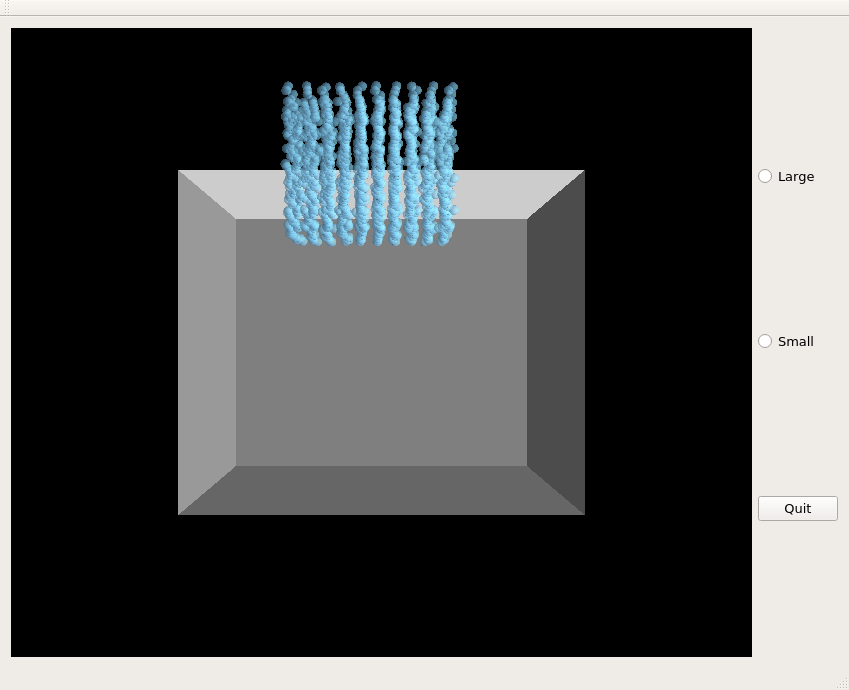
\includegraphics[width=\columnwidth,natwidth=2in,natwidth=3in]{image4.png}
\end{figure}
\begin{figure}[h]
  \caption{1000 particles after collisions}
  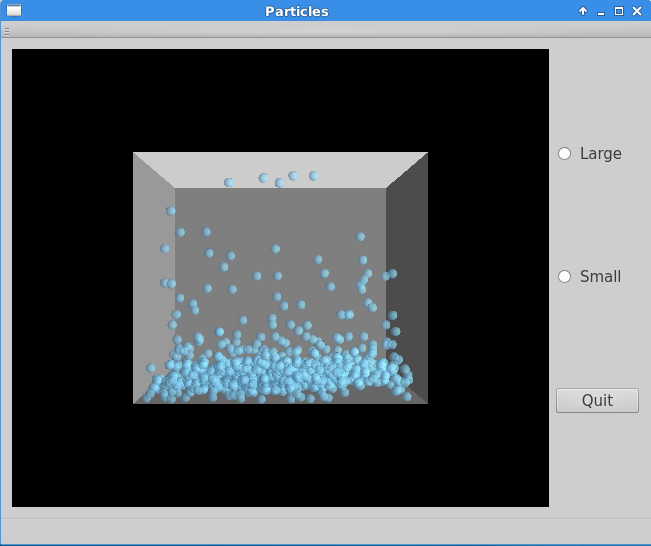
\includegraphics[width=\columnwidth,natwidth=2in,natwidth=3in]{image1.png}
\end{figure}
\begin{figure}[h]
  \caption{1000 particles after rotation}
  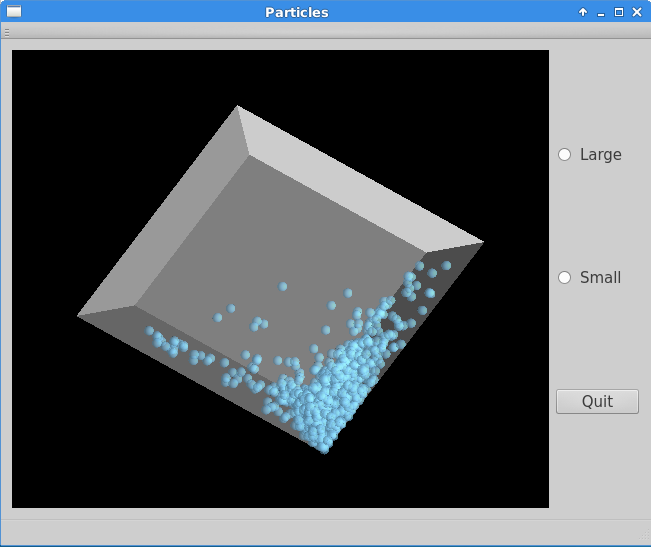
\includegraphics[width=\columnwidth,natwidth=2in,natwidth=3in]{image3.png}
\end{figure}
\begin{figure}[h]
  \caption{larger particles after collisions}
  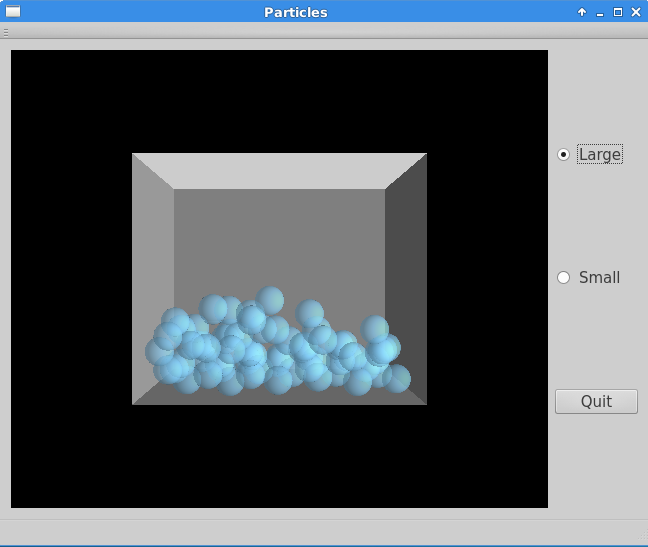
\includegraphics[width=\columnwidth,natwidth=2in,natwidth=3in]{image2.png}
\end{figure}
